\section{Kravspecifikation}
\subsection{Indledning}
\subsection{Ordliste}
\subsubsection{Aktivitet} En opgave med tilknyttet varighed, medarbejdere kan deltage i at udføre.
\subsubsection{Faste aktiviteter} Aktiviteter der ikke kan pålægges et projekt. F.eks. ferie, sygdom, kurser.
\subsubsection{Projekt aktivitet}
\subsubsection{Projekt} Samling af aktiviteter, er internt (dvs. at projektet er Softwarehuset A/S' eget) eller ikke-internt (for en kunde).
\subsubsection{Medarbejder} Alias udviklingsmedarbejder; de som står for udviklingen af softwareløsninger til kunder.
\subsubsection{Kunde}
\subsubsection{Projektleder} En medarbejder valgt blandt udviklingsmedarbejdere
\subsubsection{Softwarehuset A/S} Kunden til softwareløsningen
\subsubsection{Medarbejder} Identifikation	Initialer på 4 bogstaver. F.eks. huba
\subsubsection{Projektnumre} Har formen årstal og et løbenummer. F.eks. 22001
\subsubsection{Varighed} En aktivitets fastlagte antal timer
\subsubsection{Arbejdstid} Mængde tid i inkrementer af halve timer, brugt på en aktivitet


\subsection{Use case diagrams}

\subsubsection{Projektstyring} 

\begin{figure}[ht]
    \centering
    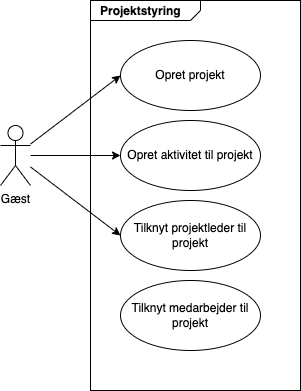
\includegraphics{diagrams/guest_project}
    \caption{Use case: Projektstyring}
    \label{fig:my_image}
\end{figure}

\subsubsection{Aktivitetshåndtering}
\begin{figure}[ht]
    \centering
    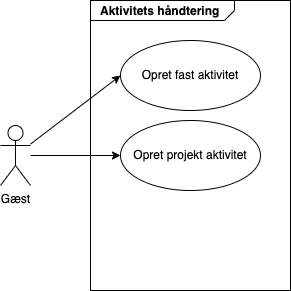
\includegraphics{diagrams/guest_activity}
    \caption{Use case: Aktivitetshåndtering}
    \label{fig:my_image}
\end{figure}


\subsubsection{Bruger administration} 
\begin{figure}[ht]
    \centering
    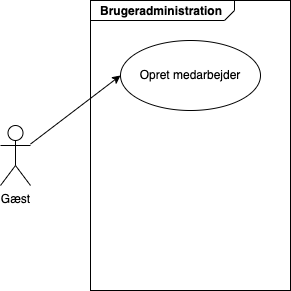
\includegraphics{diagrams/guest_users}
    \caption{Use case: Brguer administration}
    \label{fig:my_image}
\end{figure}

\subsection{Detaljerede use cases}

\subsection{Opret projekt}


\Large{Kaspers udkast af use case}

\normalsize
\underline{Navn} \\
Opret projekt

\underline{Beskrivelse} \\
Der kan oprettes projekter

\underline{Aktør} \\
Bruger

\begin{figure}
    \centering
    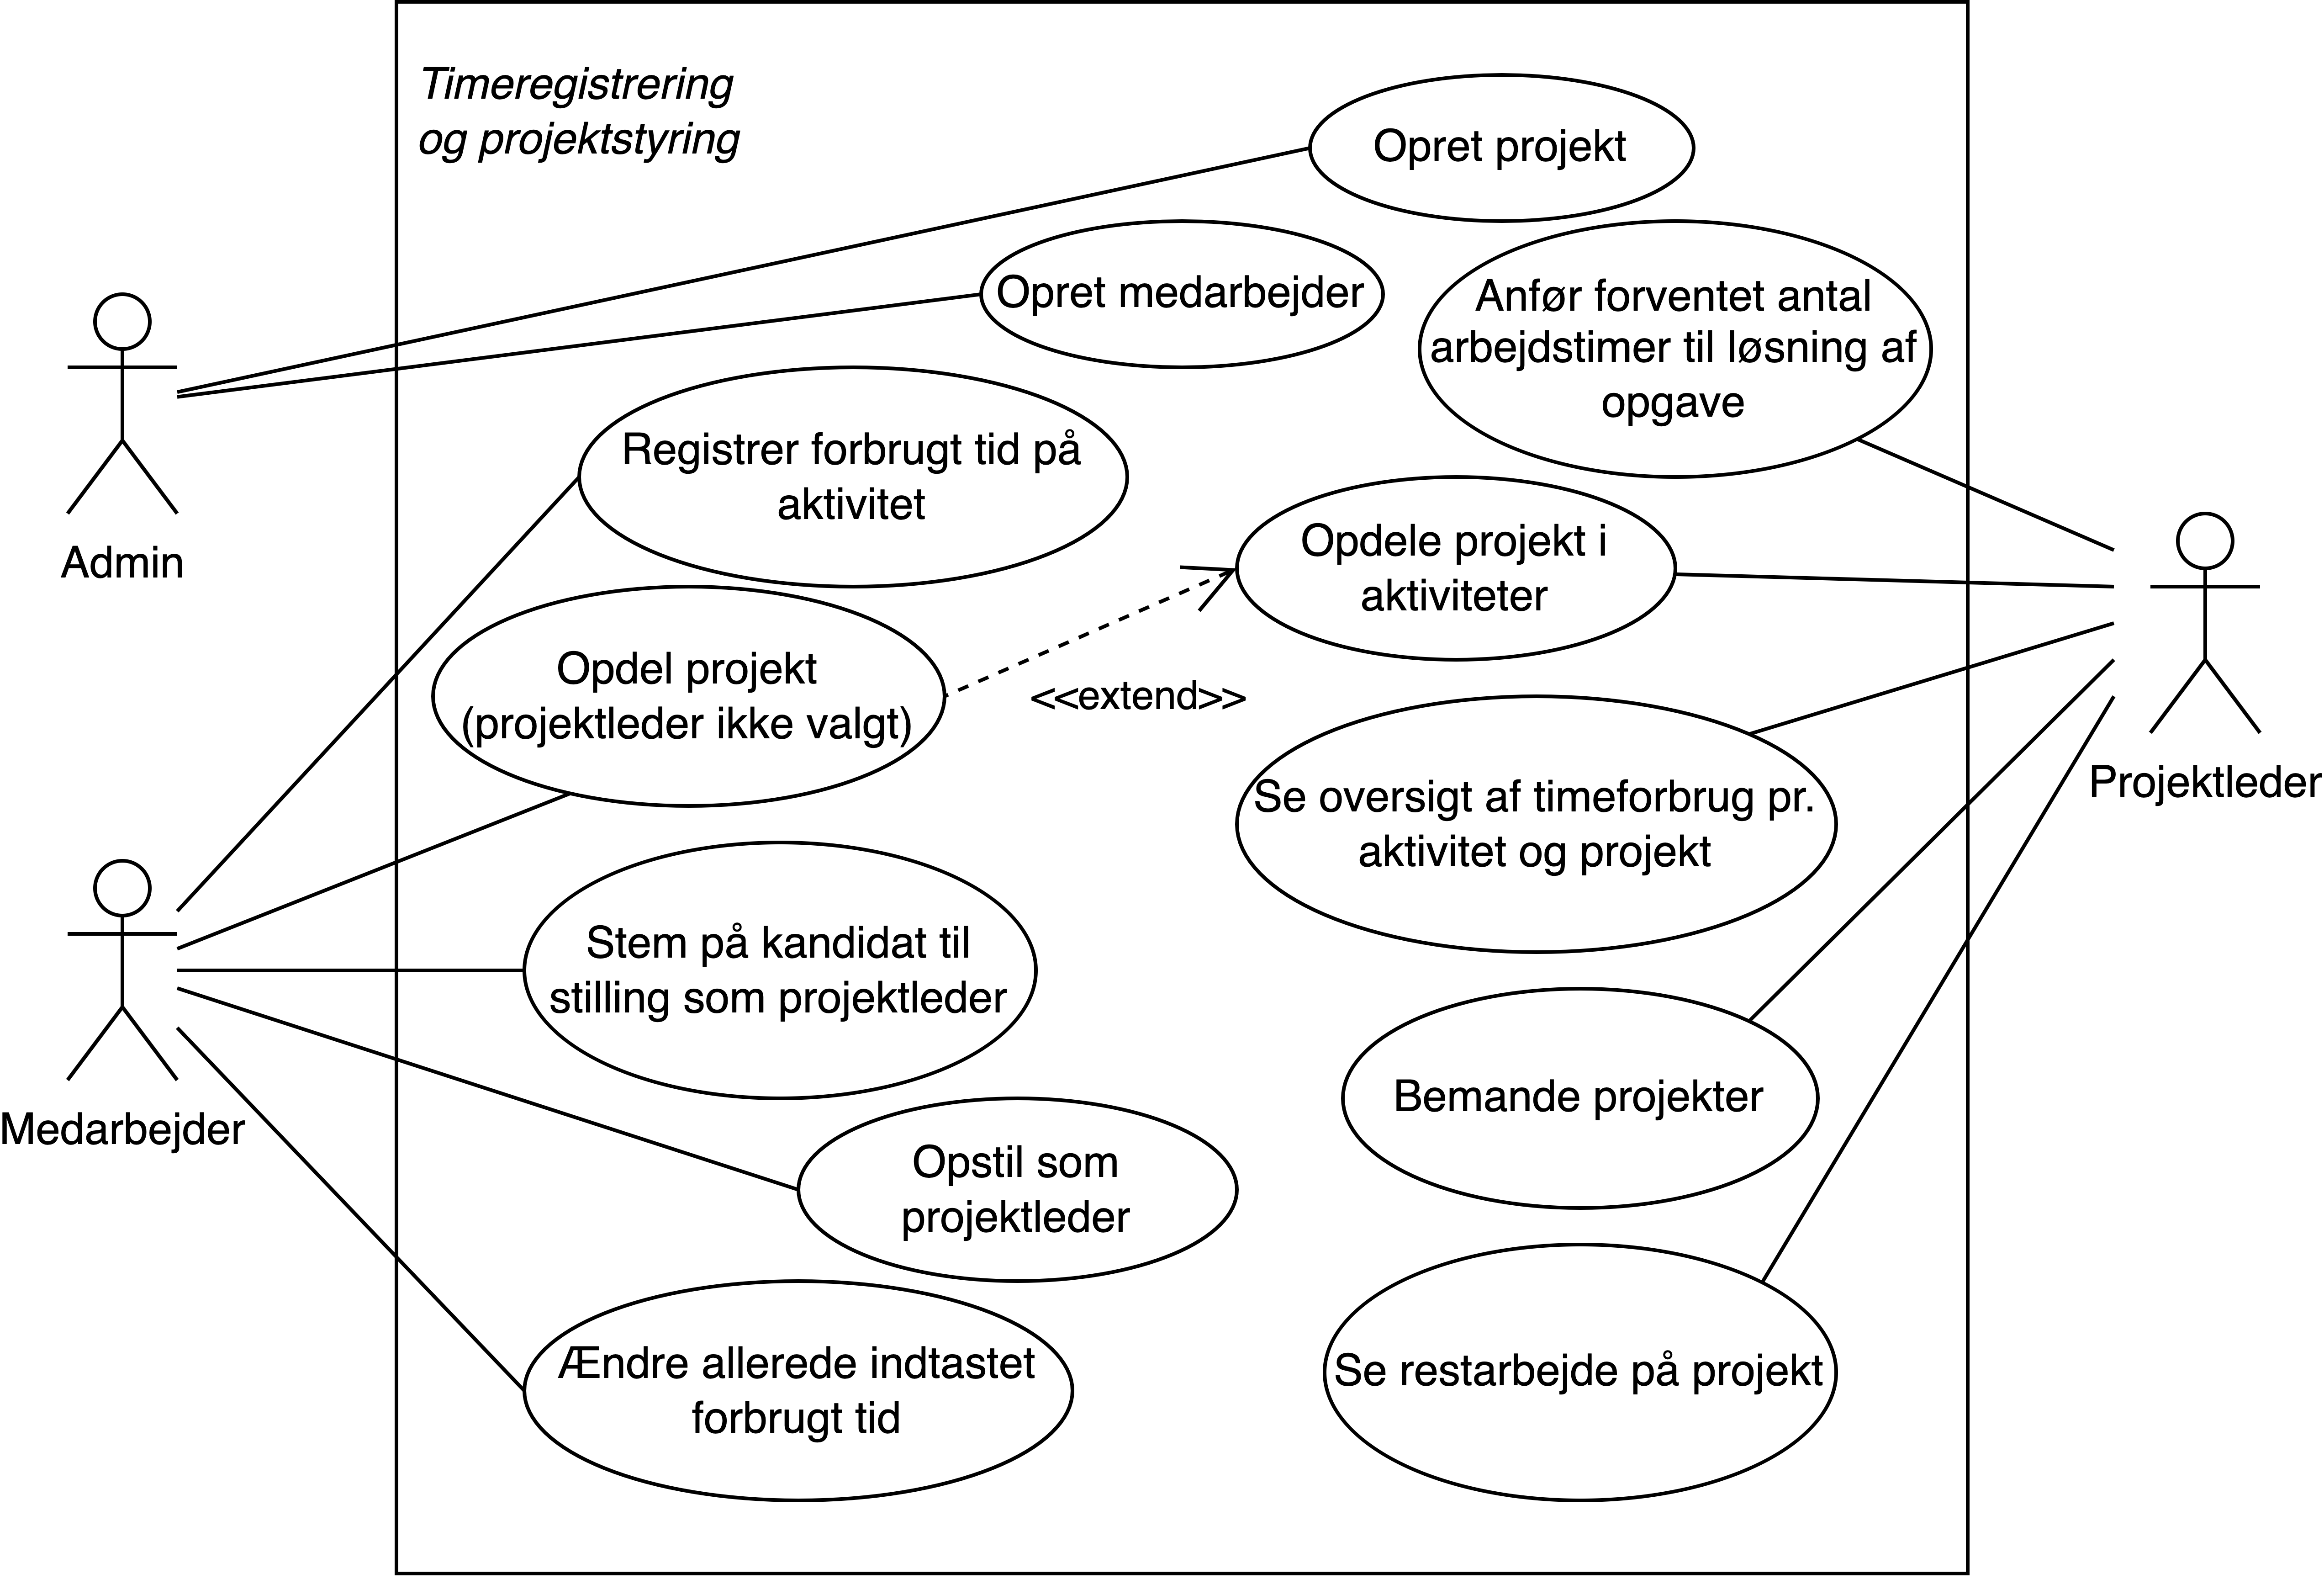
\includegraphics{RequirementsAndDesign/diagrams/Timeregistrering og projektstyring.png}
    \caption{Det her var et forsøg på at lave et use-case diagram med alle actors tilstede. Der er muligvis også flere use-cases end nødvendig, men de her er stillet af opgaven, som fremgår af projektbeskrivelsen. Ikke nødvendigvis det mest overskuelige use-case diagram, men en fordel ved denne er - selvom det er en mindre detalje - at man får en enkel use-case relation med, nemlig <<extend>>. (Mathies)}
    \label{AlleActorsPåEnGang}
\end{figure}

\underline{Cucumber feature 1}
\begin{verbatim}
Feature: Buy fruit
Description: A user buys fruit...
Actors: User

Scenario: Buy a fruit with enough money
    Given the vending machine has fruits
    When the user enters enough mone for a fruit
    And the user selects a fruit
    And the machine returns the rest money
    And the vending machine remembers its earnings
    ...
    
\end{verbatim}
